% meta.concepts: 2D rigid-body force equilibrium
% meta.tags: realistic
% acknowledge: Peter Seiler & Luke Melander graciously shared Spring 2019 course material
% source: 2019 P. Seiler AEM2011 HW 5


The engineers constructing the famous cherry and spoon sculpture in Minneapolis were required to carry out a
structural analysis in case of an earthquake. They conducted the analysis by assuming that after an earthquake
the foundation was not able to provide any rigid support to the structure. This means that the structure is
just resting on the ground. A picture and diagram for the situation is shown below. Assume that:
\begin{itemize}
  \item The mass of section ABC is 100 kg and the weight acts at point B.
  \item The mass of section CD is 80 kg and the weight acts at the mid-point of CD.
  \item The mass of the cherry is 100 kg and the cherry is placed at a distance $d$ from the point C.
  \item Point C acts as a hinge while A acts as roller support.
\end{itemize}
Complete the following analyses:
\begin{enumerate}
  \item Find the maximum value of distance d such that the system does not topple about point C.
  \item The ground at A can only support a load of 300 N. What is the minimum value of distance $d$ such that
the normal reaction force at point A does not exceed 300 N?
\end{enumerate}

\begin{figure}[ht!]
  \centering
  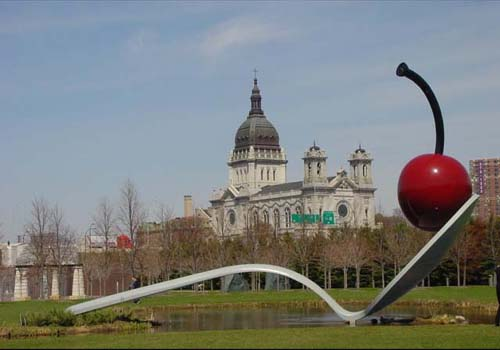
\includegraphics[height=1.5in]{figa.png}
  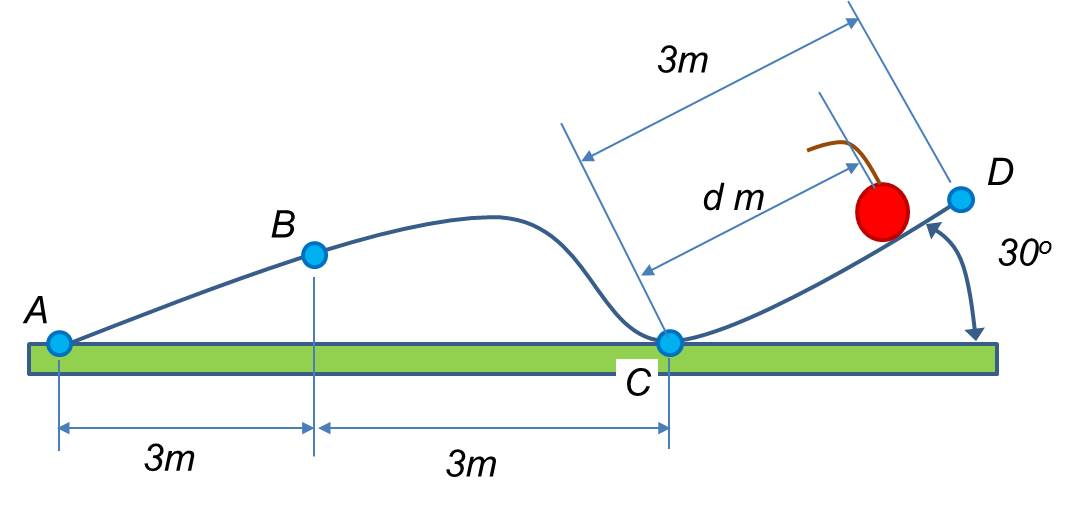
\includegraphics[height=1.5in]{figb.png}
\end{figure}

\iftoggle{flagSoln}{%
\vspace{.5cm}
\rule{\textwidth}{.4pt}
\vspace{.5cm}
\textbf{Solution:}
\begin{figure}[ht!]
  \centering
  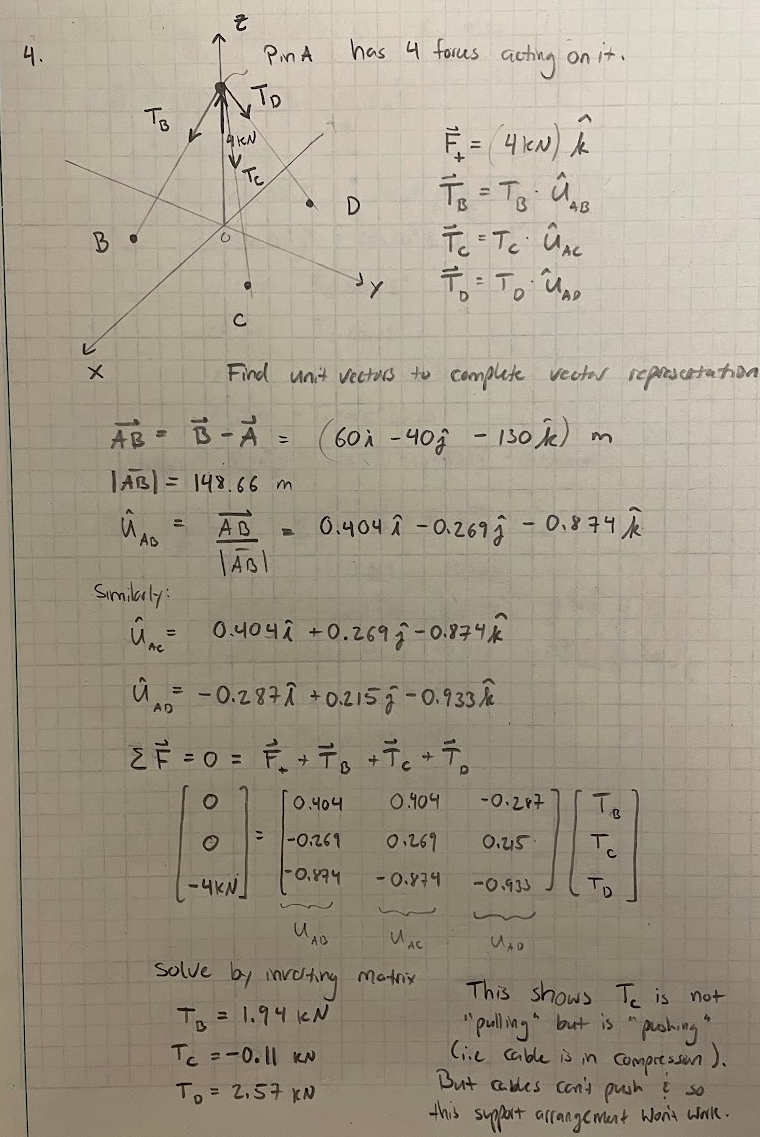
\includegraphics[width=0.9\textwidth,
	           height=0.3\textheight,
		   keepaspectratio]{soln.png}
\end{figure}
}{%
}%
